\vspace{-0.35cm}
\subsection{Our Approach for Scaling Offline RL}
\label{sec:scaledql_method}
\vspace{-0.3cm}

In this section, we describe the important architectural design decisions required to make offline CQL effective in learning highly-expressive neural network policies from large offline datasets. 

\begin{figure}[t]
    \centering
    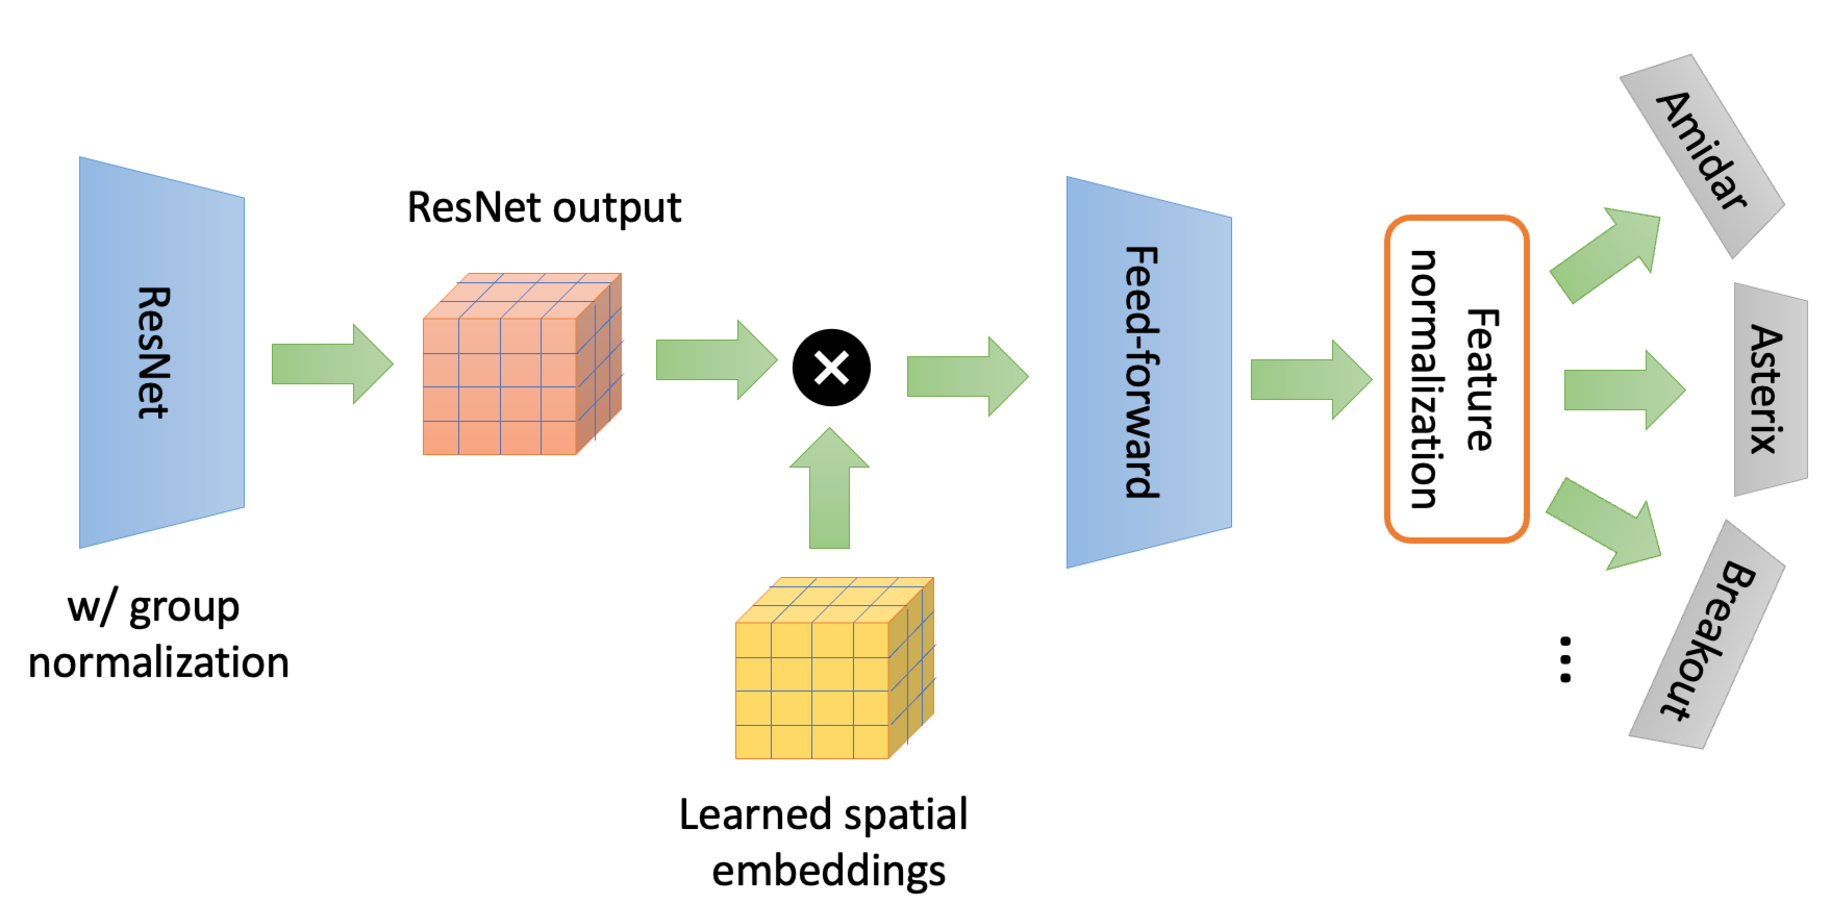
\includegraphics[width=0.6\linewidth]{chapters/scaled_ql/figures/network_figure.pdf}
    \vspace{-0.3cm}
    \caption{\footnotesize{\textbf{An overview of the network architecture.} The key design decisions are: (1) the use of ResNet models with learned spatial embeddings and group normalization, (2) use of a distributional representation of return values and cross-entropy TD loss for training (i.e., C51~\citep{bellemare2017distributional}), and (3) feature normalization to stablize training.}}
    \label{fig:architecture}
    \vspace{-0.3cm}
\end{figure}
\textbf{Parameterization of Q-values and TD error.} In the single game setting, both mean-squared TD error and distributional TD error perform comparably online~\citep{agarwal2021deep} and offline~\citep{kumar2020conservative,kumar2021dr3}. In contrast,  
we observed, perhaps surprisingly, that mean-squared TD error does not scale well, and performs much worse than using a \textcolor{brown}{\textbf{categorical distributional representation of return values}}~\citep{bellemare2017distributional} when we train on many Atari games. We hypothesize that this is because even with reward clipping, Q-values for different games often span different ranges, and training a single network with shared parameters to accurately predict all of them presents challenges pertaining to gradient interference along different games~\citep{hessel2019popart, yu2020gradient}. 
While prior works have proposed to use adaptive normalization schemes~\citep{hessel2019popart,kurin2022defense}, preliminary experiments with these approaches were not effective to close the gap. 

\textbf{Q-function architecture.} 
Since large neural networks has been crucial for scaling to large, diverse datasets in NLP and vision~\citep[e.g.,][]{tan2019efficientnet, brown2020language, kaplan2020scaling}, we explore using bigger architectures for scaling offline Q-learning. We use standard feature extractor backbones from vision, namely, the Impala-CNN architectures~\citep{espeholt2018impala} that are fairly standard in deep RL and ResNet $34$, $50$ and $101$ models from the ResNet family~\citep{resnet}. We make modifications to these networks following certain recommendations from robotic RL (see Chapter~\ref{chapter:ptr} for a detailed discussion of these changes): we utilize group normalization instead of batch normalization in ResNets, and utilize point-wise multiplication with a learned spatial embedding when converting the output feature map of the vision backbone into a flattened vector which is to be fed into the feed-forward part of the Q-function. 

To handle the multi-task setting, we use a multi-headed architecture where the Q-network outputs values for each game separately. The architecture uses a shared encoder and feedforward layers with separate linear projection layers for each game (Figure~\ref{fig:architecture}). The training objective of CQL is computed using the Q-values for the game that the transition originates from. 

\textbf{{Feature Normalization via DR3.}}
Our preliminary experiments with the design decisions discussed above on a subset of games did not attain good performance. In the single-task setting, the DR3 regularizer that stabilizes training and allows the network to better use capacity, however, as we discussed in Section~\ref{sec:dr3_section}, it introduces an additional hyperparameter to tune. To alleviate this bottleneck, we utilize the normalization variant of DR3 for our large-scale experiments, and regularize the magnitude of the learned features of the observation to have an $\ell_2$ norm of 1 by construction. We present an ablation study analyzing this choice in Table~\ref{tab:ablation_dr3} and find that indeed DR3 normalization improves performance across the board. 
% We found this sufficient to achieve strong performance, however, we leave exploring alternative feature regularization schemes to future work.

\begin{tcolorbox}[colback=blue!6!white,colframe=black,boxsep=0pt,top=3pt,bottom=5pt]
\textbf{To summarize,} the primary modifications that enable us to scale CQL are: \textbf{(1)} use of large ResNets with learned spatial embeddings and group normalization,
\textbf{(2)} use of a distributional representation of return values and cross-entropy loss for training (i.e., C51~\citep{bellemare2017distributional}), and \textbf{(3)} feature normalization at intermediate layers via DR3 to prevent feature co-adaptation (Section~\ref{sec:dr3_section}). We call our approach \textbf{Scaled Q-learning}.
\end{tcolorbox} 
